\documentclass[12pt]{article}

\usepackage{tikz}
\usepackage{amsmath}
\usepackage{amssymb}
\usepackage[super]{nth}
\usepackage{subcaption}
\usepackage{gensymb}

\usepackage{hyperref}
\hypersetup{
	colorlinks,
	citecolor=black,
	filecolor=black,
	linkcolor=black,
	urlcolor=black
}

\usepackage{needspace}
\usepackage{xpatch}
%\xpretocmd{\section}{{\needspace{20\baselineskip}{}{}
\xpretocmd{\subsection}{\needspace{15\baselineskip}}{}{}
\xpretocmd{\subsubsection}{\needspace{10\baselineskip}}{}{}

\title{Counting Lattice Paths}
\author{Frank Rodriguez}
\date{May \nth{4}, 2018}

\newcommand{\p}{\paragraph{}}
\captionsetup{format=hang}
\newcommand{\grid}[2]{\tikz \draw[scale=.5] grid (#1, #2);}
\newcommand{\fall}[1]{\strut^{\underline{#1}}}

\begin{document}
	\pagenumbering{gobble}
	\maketitle
	\newpage
	
	\pagenumbering{roman}
	\tableofcontents
	\newpage
	\pagenumbering{arabic}
	
	\section{Introduction}
	
		\begin{figure}[h]
			\centering
			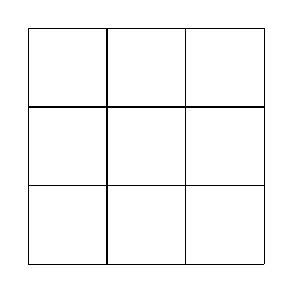
\begin{tikzpicture}[scale=1]
				\draw grid (3,3);
			\end{tikzpicture}
			
			\caption{A lattice}
		\end{figure}
		
		\p This is a lattice. They are different from grids in that our focus is not on the squares themselves, but rather on the corners and edges. In the system we will discuss in this paper, the goal is to travel along the edges from the top left corner to the bottom right corner. However, there are only two legal moves: moving right, and moving down. Here are some example legal paths:
		
		\begin{figure}[h]
			\centering
			\begin{subfigure}{.3\textwidth}
				\centering
				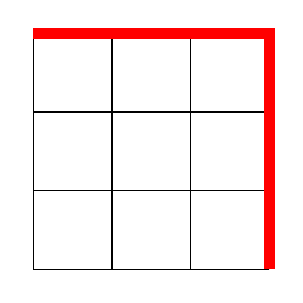
\begin{tikzpicture}[scale=1]
				\draw grid (3,3);
				\draw [line width=4, red] (0,3) --(3,3) --(3,0);
				\end{tikzpicture}
			\end{subfigure}%
			\begin{subfigure}{.3\textwidth}
				\centering
				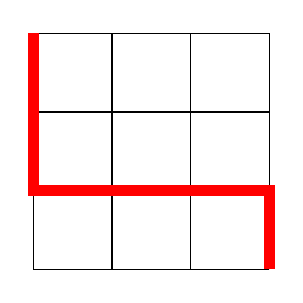
\begin{tikzpicture}[scale=1]
				\draw grid (3,3);
				\draw [line width=4, red] (0,3) --(0,1) --(3,1) --(3,0);
				\end{tikzpicture}
			\end{subfigure}%
			\begin{subfigure}{.3\textwidth}
				\centering
				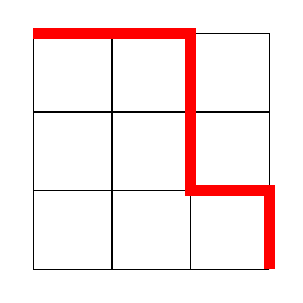
\begin{tikzpicture}[scale=1]
				\draw grid (3,3);
				\draw [line width=4, red] (0,3) --(2,3) --(2,1) --(3,1) --(3,0);
				\end{tikzpicture}
			\end{subfigure}
		
			\caption{A few lattice paths}
		\end{figure}
	
		\newpage
		\p And here are some illegal paths:
		
		\begin{figure}[h]
			\centering
			\begin{subfigure}{.3\textwidth}
				\centering
				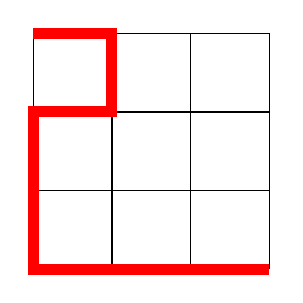
\begin{tikzpicture}[scale=1]
				\draw grid (3,3);
				\draw [line width=4, red] (0,3) --(1,3) --(1,2) --(0,2) --(0,0) --(3,0);
				\end{tikzpicture}
			\end{subfigure}%
			\begin{subfigure}{.3\textwidth}
				\centering
				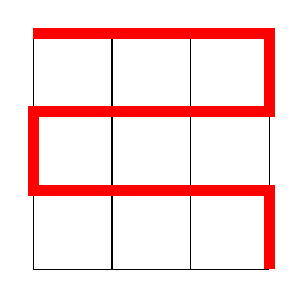
\begin{tikzpicture}[scale=1]
				\draw grid (3,3);
				\draw [line width=4, red] (0,3) --(3,3) --(3,2) --(0,2) --(0, 1) --(3, 1) --(3, 0);
				\end{tikzpicture}
			\end{subfigure}%
			\begin{subfigure}{.3\textwidth}
				\centering
				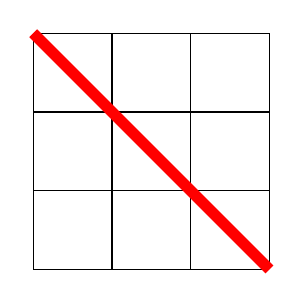
\begin{tikzpicture}[scale=1]
				\draw grid (3,3);
				\draw [line width=4, red] (0,3) --(3,0);
				\end{tikzpicture}
			\end{subfigure}
			
			\caption{Some illegal lattice paths}
		\end{figure}
	
		\p The question then becomes, given any lattice, how can we calculate the number of legal paths it contains?
	
	\section{Counting}
	
		\subsection{Simple Counting}
			
			\p The first idea one might have is to simply count the number of paths in a lattice by hand. There is nothing particularly flawed about this approach, and it can technically be used to solve any lattice. For example, here are the paths of a one-by-one lattice:
			
			\begin{figure}[h]
				\centering
				\begin{subfigure}{.5\textwidth}
					\centering
					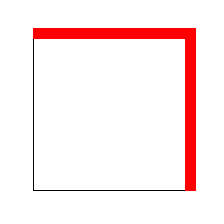
\begin{tikzpicture}[scale=2]
						\draw grid (1,1);
						\draw [line width=4, red] (0,1) --(1,1) --(1,0);
					\end{tikzpicture}
				\end{subfigure}%
				\begin{subfigure}{.5\textwidth}
					\centering
					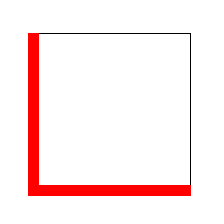
\begin{tikzpicture}[scale=2]
					\draw grid (1,1);
					\draw [line width=4, red] (0,1) --(0,0) --(1,0);
					\end{tikzpicture}
				\end{subfigure}
			
				\caption{Counting all paths in a $1\times1$ lattice}
			\end{figure}
		
			\p Thus demonstrating that a $1\times1$ lattice has two paths. We will write this as $|1\times1|=2$, or ``the magnitude of a one-by-one lattice is two.'' We can repeat this to solve for $|2\times2|$:
			
			\begin{figure}[h]
				\centering
				\begin{subfigure}{.3\textwidth}
					\centering
					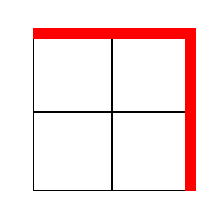
\begin{tikzpicture}[scale=1]
					\draw grid (2,2);
					\draw [line width=4, red] (0,2) --(2,2) --(2,0);
					\end{tikzpicture}
				\end{subfigure}%
				\begin{subfigure}{.3\textwidth}
					\centering
					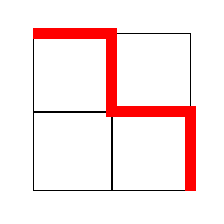
\begin{tikzpicture}[scale=1]
					\draw grid (2,2);
					\draw [line width=4, red] (0,2) --(1,2) --(1,1) --(2, 1) --(2,0);
					\end{tikzpicture}
				\end{subfigure}%
				\begin{subfigure}{.3\textwidth}
					\centering
					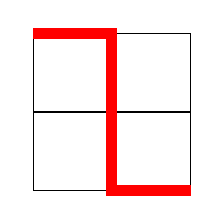
\begin{tikzpicture}[scale=1]
					\draw grid (2,2);
					\draw [line width=4, red] (0,2) --(1,2) --(1,0) --(2,0);
					\end{tikzpicture}
				\end{subfigure}\\ \vspace{1cm}%
				\begin{subfigure}{.3\textwidth}
					\centering
					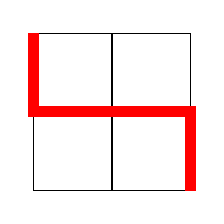
\begin{tikzpicture}[scale=1]
					\draw grid (2,2);
					\draw [line width=4, red] (0,2) --(0,1) --(2,1) --(2,0);
					\end{tikzpicture}
				\end{subfigure}%
				\begin{subfigure}{.3\textwidth}
					\centering
					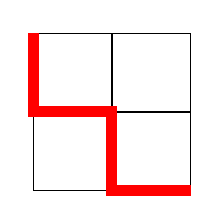
\begin{tikzpicture}[scale=1]
					\draw grid (2,2);
					\draw [line width=4, red] (0,2) --(0,1) --(1,1) --(1,0) --(2,0);
					\end{tikzpicture}
				\end{subfigure}%
				\begin{subfigure}{.3\textwidth}
					\centering
					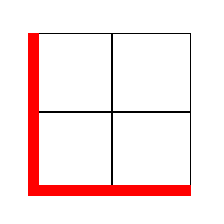
\begin{tikzpicture}[scale=1]
					\draw grid (2,2);
					\draw [line width=4, red] (0,2) --(0,0) --(2,0);
					\end{tikzpicture}
				\end{subfigure}
				
				\caption{Counting all paths in a $2\times2$ lattice}
				\label{fig:count2x2}
			\end{figure}
		
			\p This shows all six potential paths to solving our two-by-two lattice problem. What of a three-by-three lattice? While certainly possible to count all solution paths, it becomes quite easy to fumble. For even larger lattices, this becomes especially true. A better method of counting lattice paths is necessary.
			
		\subsection{Law of Reduction}
		
			\p Let us analyze a specific lattice case, the $n\times1$ lattice. By starting small, we can count their paths with little difficulty and search for patterns. Starting with a $1\times1$ lattice, we see that it has two paths. If we append a square to it in order to create a $2\times1$ lattice, what changes?
			
			\begin{figure}[h]
				\centering
				
				\begin{subfigure}{.3\textwidth}
					\centering
					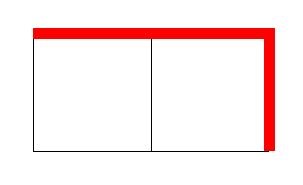
\begin{tikzpicture}[scale=1.5]
						\draw grid (2,1);
						\draw [line width=4, red] (0,1) --(2,1) --(2,0);
					\end{tikzpicture}
				\end{subfigure}%
				\begin{subfigure}{.3\textwidth}
					\centering
					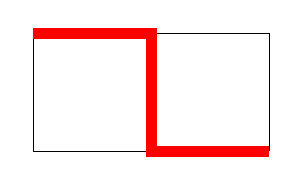
\begin{tikzpicture}[scale=1.5]
						\draw grid (2,1);
						\draw [line width=4, red] (0,1) --(1,1) --(1,0) --(2,0);
					\end{tikzpicture}
				\end{subfigure}%
				\begin{subfigure}{.3\textwidth}
					\centering
					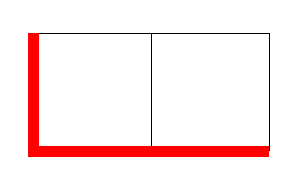
\begin{tikzpicture}[scale=1.5]
						\draw grid (2,1);
						\draw [line width=4, red] (0,1) --(0,0) --(2,0);
					\end{tikzpicture}
				\end{subfigure}
			
				\caption{Counting all paths in a $2\times1$ lattice}
			\end{figure}
		
			\p While $|1\times1|$ is two, it seems as though adding another square added only a single path. Why is this?
			
			\p In the $1\times1$ lattice, the only two paths were the outermost paths. As we are dealing with rectangular paths (paths which can be fully described as $n\times p$), there will \emph{always} be two outermost paths available. Thus, the $2\times1$ lattice also has these same two options. However, it has one new option -- the edge formed where one square touches the other.
			
			\p This explains why only one path was added when a new square was added. In fact, this pattern can be seen persisting as we add more and more squares to the lattice:
			
			\begin{figure}[h]
				\centering
				\captionsetup[subfigure]{justification=justified,singlelinecheck=false}
				
				\begin{subfigure}{.5\textwidth}
					
					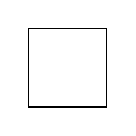
\begin{tikzpicture}
						\draw grid (1,1);
					\end{tikzpicture}
					\caption*{$|1\times1|=2$}
				\end{subfigure}\hfill%
				%
				\begin{subfigure}{.5\textwidth}
					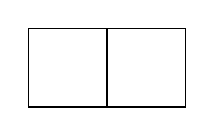
\begin{tikzpicture}
						\draw grid (2,1);
					\end{tikzpicture}
					\caption*{$|2\times1|=3$}
				\end{subfigure}\\ \vspace{.5cm}%
				%
				\begin{subfigure}{.5\textwidth}
					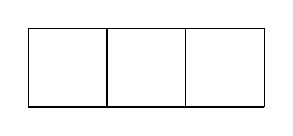
\begin{tikzpicture}
						\draw grid (3,1);
					\end{tikzpicture}
					\caption*{$|3\times1|=4$}
				\end{subfigure}\hfill%
				%
				\begin{subfigure}{.5\textwidth}
					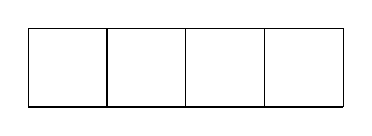
\begin{tikzpicture}
						\draw grid (4,1);
					\end{tikzpicture}
					\caption*{$|4\times1|=5$}
				\end{subfigure}\\ \vspace{.5cm}%
				%
				\begin{subfigure}{.5\textwidth}
					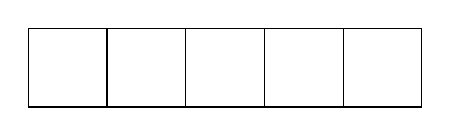
\begin{tikzpicture}
						\draw grid (5,1);
					\end{tikzpicture}
					\caption*{$|5\times1|=6$}
				\end{subfigure}\hfill%
				%
				\begin{subfigure}{.5\textwidth}
					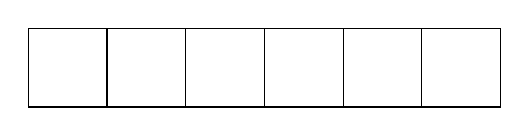
\begin{tikzpicture}
						\draw grid (6,1);
					\end{tikzpicture}
					\caption*{$|6\times1|=7$}
				\end{subfigure}\\ \vspace{.5cm}
				
				\caption{Succession of paths in $n\times1$ lattices}
			\end{figure}
		
			\p The general pattern becomes clear, and we can generalize this rule to come up with our first ``lattice law.'' These will be a set of tools which will help us analyze lattices:
			
			\begin{equation*}
				|n \times 1| = n + 1
			\end{equation*}
			
		\subsection{Law of Symmetry}
		
			\p What if we rotate our lattices? Since they are rectangular, rotations of $180\degree$ will have no effect on the lattice -- it would be indistinguishable from the original orientation. Therefore, only rotations $90\degree$ clockwise or counterclockwise need to be considered.
			
			\p Square lattices are the exception, as any rotation would leave them indistinguishable from its original position.\footnote{We only consider rotations in increments of $90\degree$. In the context of the pathing problem we are solving, no other type of rotation makes sense.} We will start with the $2\times1$ lattice. Notice how rotating it $90\degree$, be it clockwise or counterclockwise, results in the same shape of lattice -- a $1\times2$ lattice (indeed, this is always the case):
			
			\begin{figure}[h]
				\centering
				
				\begin{subfigure}{.3\textwidth}
					\centering
					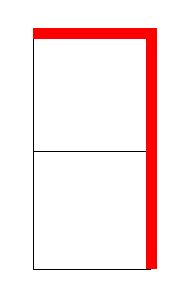
\begin{tikzpicture}[scale=1.5]
					\draw grid (1,2);
					\draw [line width=4, red] (0,2) --(1,2) --(1,0);
					\end{tikzpicture}
				\end{subfigure}%
				\begin{subfigure}{.3\textwidth}
					\centering
					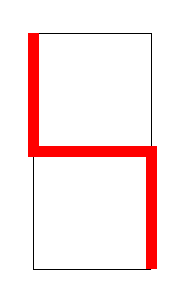
\begin{tikzpicture}[scale=1.5]
					\draw grid (1,2);
					\draw [line width=4, red] (0,2) --(0,1) --(1,1) --(1,0);
					\end{tikzpicture}
				\end{subfigure}%
				\begin{subfigure}{.3\textwidth}
					\centering
					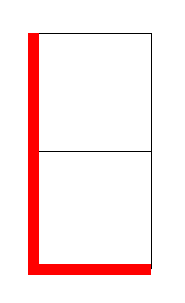
\begin{tikzpicture}[scale=1.5]
					\draw grid (1,2);
					\draw [line width=4, red] (0,2) --(0,0) --(1,0);
					\end{tikzpicture}
				\end{subfigure}
				
				\caption{Counting all paths in a $1\times2$ lattice}
			\end{figure}
		
			\p The $1\times2$ lattice had three paths, and it appears that the $2\times1$ lattice also has three paths. Why?
			
			\p We can represent a rotation as a switch in the placement of the numbers in the notation. In other words, a rotation of $n \times p$ can be written as $p \times n$. Note that, if $n \neq p$, then this new lattice is \emph{not} the same as the original lattice, but do realize what the rotation has done. After rotation, all right path steps became down path steps, and all down path steps became right path steps. By writing out the rotation in terms of $n \times p$, this is much easier to see.
			
			\p The significance of this is that, while $n \times p$ is not the same lattice as $p \times n$ for all $n \neq p$, the number of paths in the two lattices is the same. This gives us our second lattice law:
			
			\begin{equation*}
				|n \times p| = |p \times n|
			\end{equation*}
			
			\p This proves that our first lattice law applies to its rotated forms. In other words, because $|n \times 1| = n+1$ is true, then $|1 \times n| = n + 1$ must also be true. It might be helpful to then reconsider our first lattice law to be:
			
			\begin{equation*}
				|n \times 1| = |1 \times n| = n + 1
			\end{equation*}
			
	\section{Advanced Counting}
	
		\subsection{Lattice Decomposition}
			
			\p So far, we have two lattice laws:
			
			\begin{align*}
				|n \times 1| &= n + 1 \\
				|n \times p| &= |p \times n|
			\end{align*}
			
			\p This helps us solve very easy lattices, but is still not powerful enough to tackle more complex ones. Consider our $2 \times 2$ lattice:
			
			\begin{figure}[h]
				\centering
				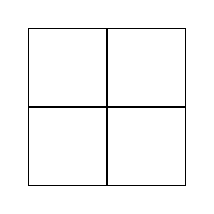
\begin{tikzpicture}
					\draw grid (2,2);
				\end{tikzpicture}
				
				\caption{A $2 \times 2$ lattice.}
			\end{figure}
		
			\p We cannot count the number of paths it contains using \emph{only} our lattice laws. We need a method of turning these larger lattices into more manageable chunks.
			
			\p In order to do this, we need a realization. What happens when you move right?
			
			\begin{figure}[h]
				\centering
				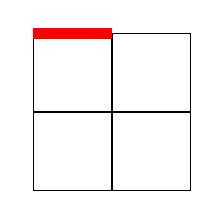
\begin{tikzpicture}
				\draw grid (2,2);
				\draw [line width=4, red] (0,2) --(1,2);
				\end{tikzpicture}
				
				\caption{One step right.}
			\end{figure}
		
			\p Once you take a step to the right, you cannot move back, as left steps are not legal. Thus, when you move right, all possible paths are contained within the right side of the lattice:
			
			\begin{figure}[h]
				\centering
				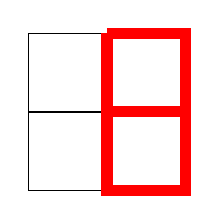
\begin{tikzpicture}
				\draw grid (2,2);
				\draw [line width=4, red] (1,2) --(2,2) --(2,0) --(1,0) --(1,2);
				\draw [line width=4, red] (1,1) --(2,1);
				\end{tikzpicture}
				
				\caption{All possible consequences of moving right once.}
			\end{figure}
		
			\p Likewise, when you take a step down, all possible paths this can lead to are contained within the lower part of the lattice:
			
			\begin{figure}[h]
				\centering
				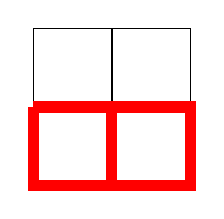
\begin{tikzpicture}
				\draw grid (2,2);
				\draw [line width=4, red] (0,1) --(2,1) --(2,0) --(0,0) --(0,1);
				\draw [line width=4, red] (1,1) --(1,0);
				\end{tikzpicture}
				
				\caption{All possible consequences of moving down once.}
			\end{figure}
		
			\p Because these two pieces of the lattice contain all consequences to the final path from our first move, and because these two sets of paths are independent of each other, we can say that the whole lattice's paths are the sum of these two sub-lattice's paths.
			
			\p When you move to the right, you end up with a $1 \times 2$ lattice. By the first law, this has three paths. When you move down, you end up with a $2\times1$ lattice. Again by the first law, this has three more paths.
			
			\p Thus, $|2\times2| = |1\times2| + |2\times1| = 3 + 3 = 6$, and indeed this is what we counted earlier (figure \ref{fig:count2x2}).
			
			\p We can generalize this further. Moving to the right in an $n \times p$ results in a sub-lattice which has the leftmost edge cut off. This is equivalent to an $(n-1) \times p$ lattice.
			
			\p Likewise, moving down in an $n \times p$ lattice produces a sub-lattice which has the top row cut off. This is equivalent to an $n \times (p-1)$ lattice.
			
			\p This pair of sub-lattices represents all possible paths in the parent lattice, giving us our third lattice law:
			
			\begin{equation*}
				|n \times p| = |(n-1) \times p| + |n \times (p-1)|
			\end{equation*}
			
			\p Combined with the first two laws, we now have a high enough understanding of lattices to count the number of paths in more difficult configurations.
			
		\subsection{Worked Example: $|3 \times 3|$}
		
			\p First, a reminder of our lattice laws:
			
			\begin{align*}
				|n \times 1| &= n + 1\\
				|n \times p| &= |p \times n| \\
				|n \times p| &= |(n-1) \times p| + |n \times (p - 1)|
			\end{align*}
			
			\p Given this, counting the paths in a $3\times3$ lattice can be done graphically:
			
			\begin{figure}[h]
				\centering
				
				\begin{tikzpicture}[level/.style={sibling distance=60mm/#1}]
					\node (a) {\grid{3}{3}}
					child {node (b) {\grid{2}{3}}
						child {node (c) {\grid{1}{3}}
							child {node (d) {4}}}
						child {node (e) {\grid{2}{2}}
							child {node (f) {\grid{1}{2}}
								child {node (g) {3}}}
							child {node (h) {\grid{2}{1}}
								child {node (i) {3}}}}}
					child {node (j) {\grid{3}{2}}
						child {node (k) {\grid{2}{2}}
							child {node (l) {\grid{1}{2}}
								child {node (m) {3}}}
							child {node (p) {\grid{2}{1}}
								child {node (q) {3}}}}
						child {node (n) {\grid{3}{1}}
							child {node (o) {4}}}};
				\end{tikzpicture}
				
				\caption{Graphical decomposition of a $3\times3$ lattice. The final answer is $4+3+3+3+3+4$, or $20$.}
			\end{figure}
			\newpage
		
			\p It can also be done analytically:
			
			\begin{alignat*}{2}
				|3\times3| &= |3\times2| + |2\times3| &&\qquad\text{(Decomposition)}\\
				&= 2|3\times2| &&\qquad\text{(Symmetry)}\\
				&= 2(|2\times2| + |3\times1|) &&\qquad\text{(Decomposition)} \\
				&= 2(|2\times2| + 4) &&\qquad\text{(Reduction)}\\
				&= 2(|1\times2| + |2\times1| + 4) &&\qquad\text{(Decomposition)}\\
				&= 2(2(|1\times2|) + 4) &&\qquad\text{(Symmetry)} \\
				&= 2(2(3) + 4) &&\qquad\text{(Reduction)} \\
				&= 20 &&\qquad\text{(Arithmetic)}
			\end{alignat*}
			
			\p This showcases the utility of the laws we derived. However, it also becomes unwieldy for even larger lattices, such as a $6\times6$. While this method can make tackling lattices much easier to conceptualize than simply counting paths, it is still not the best way to tackle the task.
			
	\section{A Total Solution}
		
		\subsection{The $n\times1$ Case}
			
			\p The $n\times1$ lattice case has a special property: we have a distinct formula for calculating the number of paths it contains, $|n\times1|=n+1$. As the size of the $n\times1$ lattice increases, the difficulty in counting its paths does \emph{not} increase. At a glance, we can determine that $|10,000\times1|$ is simply $10,001$, or that $|999,999,999\times1|$ is simply $1,000,000,000$. Can this seemingly unique case be applied to larger lattices?
			
			\p Take for example an $n\times2$ lattice. With our lattice laws alone, we have no shortcut, no formula that will immediately tell us the answer. We would have to decompose the lattice into smaller and smaller pieces, until we end with a series of $n\times1$ lattices, which we can then extract real numbers from. 
			
			\p When doing this, can we find a pattern? Is there something more going on than simple decomposition? Let's try solving a $6\times2$ lattice, graphically:
			
			\begin{figure}[h]
				\centering
				
				\begin{tikzpicture}[level/.style={sibling distance=65mm/#1}]
					\node {\grid{6}{2}}
						child {node {\grid{6}{1}}
							child {node {7}}}
						child {node {\grid{5}{2}}
							child {node {\grid{5}{1}}
								child {node {6}}}
							child {node {\grid{4}{2}}
								child {node {\grid{4}{1}}
									child {node {5}}}
								child {node {\grid{3}{2}}
									child {node {\grid{3}{1}}
										child {node {4}}}
									child {node {\grid{2}{2}}
										child {node {\grid{2}{1}}
											child {node {3}}}
										child {node {\grid{1}{2}}
											child {node {3}}}}}}};
				\end{tikzpicture}
				
				\caption{Graphical decomposition of a $6\times2$ lattice.}
			\end{figure}
			\newpage
		
			\p We end up with a neat little sum: $7+6+5+4+3+3$. This is even more significant when you realize that $3=2+1$, so we can rewrite the sum as $7+6+5+4+3+2+1$. This makes sense to always be the case: by the law of decomposition, decomposing any $n\times2$ lattice will result in one $n\times1$ lattice and one $(n-1)\times2$ lattice. This will continue until we end with a single $1\times2$ lattice, as we can then directly reduce it.
			
			\p Thus, we have an interesting property. We can solve any $n\times2$ lattice using a summation. In other words, $|n\times2|$ will equal the sum of all numbers counting from $1$ to $n+1$. More succinctly:
			
			\begin{equation*}
				|n\times2| = \sum_{i=1}^{n+1}i
			\end{equation*}
			
			\p The logic here is sound, and the formula terse, but we can still do better.
			
		\subsection{Sums of Sums of Sums...}
		
			\p When we look at a partial decomposition of an $n\times3$ lattice, we see another interesting pattern. For example, here is a $5 \times 3$ lattice:
			
			\begin{figure}[h]
				\centering
				
				\begin{tikzpicture}[level/.style={sibling distance=80mm/#1}]
				\node {\grid{5}{3}}
					child {node {\grid{5}{2}}}
					child {node {\grid{4}{3}}
						child {node {\grid{4}{2}}}
						child {node {\grid{3}{3}}
							child {node {\grid{3}{2}}}
							child {node {\grid{2}{3}}}}};
				\end{tikzpicture}
				
				\caption{Partial graphical decomposition of a $5\times3$ lattice.}
			\end{figure}
		
			\p We find that an $n\times3$ lattice can be broken up into a series of $n\times2$ lattices. Again this can be shown directly from decomposition, as decomposing an $n\times3$ lattice results in one $n\times2$ lattice and one $(n-1)\times3$ lattice. Each $n\times2$ lattice is a summation, as shown earlier. Thus, an $n\times3$ lattice is a summation of summations.
			
			\p As for the bounds, we end with a single $3\times2$ lattice and a single $2\times3$ lattice. However, just as with the $n\times2$ lattices, we can again think of the last term differently.
			
			\p The $2\times3$ lattice has $10$ paths. If we treated it purely as the $n\times2$ summations, we would finish the sequence with $\sum\limits_{i=1}^{3}i + \sum\limits_{i=1}^{2}i + \sum\limits_{i=1}^{1}i$, which is $10$ -- identical to what we counted. This means that it is safe to consider an $n\times3$ lattice as a summation of summations, from $1$ to $n$. In other words, our $5\times3$ lattice's paths could be written as:
			
			\begin{figure}[h]
				\begin{equation*}
				\sum_{i=1}^{6}i + \sum_{i=1}^{5}i + \sum_{i=1}^{4}i + \sum_{i=1}^{3}i + \sum_{i=1}^{2}i + \sum_{i=1}^{1}i = 56
				\end{equation*}
				
				\caption{$|5\times3|$, expanded.}
			\end{figure}
			
			
			\p The ``sum of sums'' is now very clear. We can thus think of $|n\times3|$ as being:
			
			\begin{equation*}
				|n\times3| = \sum_{j=1}^{n+1}\sum_{i=1}^{j}i
			\end{equation*}
			
			\p Similarly, an $n\times4$ lattice will decompose into a series of $n\times3$ lattices. Thus, $|n\times4|$ can be thought of as a ``sum of sums of sums'' -- quite a mouthful! 
			
			\begin{equation*}
				|n\times4| = \sum_{k=1}^{n+1}\sum_{j=1}^{k}\sum_{i=1}^{j}i
			\end{equation*} 
			
			\p The pattern continues, as an $n\times5$ lattice decomposes into a series of $n\times4$ lattice -- a sum of sums of sums of sums!
			
		\subsection{Finite Calculus}
		
			\p These sums quickly become excruciating to calculate as they increase in complexity exponentially. Alas, they bear no resemblance to our beautifully unique case of $|n\times1| = n+1$, where increasing the size has negligible effect on the complexity of the solution.
			
			\p Luckily, there is a way to extract such neat formulas from summations, a branch of mathematics known as ``Finite Calculus.'' The field is large, but we will only need to work with the parts regarding the transformation of sums of polynomials to closed-form functions. Let us look at some techniques.
			
			\subsubsection{The Falling Power}
			
				\p The first topic to cover is known as a ``falling power.'' Whereas a normal exponent is written as $a^b$, a falling exponent is written as $a\fall{b}$. Falling powers are similar to normal exponents, but they ``fall'' by subtracting $1$ each time. Consider $10\fall{5}$:
				
				\begin{equation*}
					10\fall{5} = 10 \cdot (10-1) \cdot (10-2) \cdot (10-3) \cdot (10-4) = 10(9)(8)(7)(6) = 30,240
				\end{equation*}
				
				\p Or $9\fall{3}$:
				
				\begin{equation*}
					9\fall{3} = 9 \cdot (9-1) \cdot (9-2) = 9(8)(7) = 504
				\end{equation*}
				
				\p Falling powers can be thought of as a factorial that terminates after a certain number of steps. It multiplies each number down to the power minus one: $a\fall{b} = a(a-1)(a-2)(a-3)\dots(a-(b-1))$.
				
				\p It is possible to translate regular exponents to falling exponents using something called \emph{Stirling Numbers}. While interesting, we will only need to translate $n^0$ and $n^1$ to falling powers. Luckily, $n^0$ is equal to $n\fall{0}$, and $n^1$ is equal to $n\fall{1}$.
				
			\subsubsection{The Finite Integral}
			
				\p The infinite integral of a variable to a power works as follows:
				
				\begin{equation*}
					\int x\strut^n dx = \frac{x\strut^{n+1}}{n+1}+C
				\end{equation*}
				
				\p A finite integral (also called a discrete integral) works in much the same way, but instead of an integral symbol, we are working with a finite integral symbol (which reflects the summation), and instead of a standard exponent, we are working with a falling exponent:
				
				\begin{equation*}
					\sum n\fall{k}\ \delta n = \frac{n\fall{k+1}}{k+1} + C
				\end{equation*}
				
				\p That applies to an indefinite finite integral. For a definite finite integral, there is another very important distinction between an infinite integral and a finite integral: $\sum\limits_a^b$ would sum from $a$ to $b-1$, something which is usually unwanted. Thus, if one wishes to sum from $a$ to $b$, he will have to take the finite integral from $\sum\limits_a^{b+1}$.
				
				\p As for constants, they work identically as they do in infinite integrals:
				
				\begin{figure}[h]
					\begin{align*}
					\int a\ dx &= x + C \\
					\sum a\ \delta n &= n + C
					\end{align*}
					
					\caption{Comparing the infinite and finite integrals of constants.}
				\end{figure}
				
				
		\subsection{Expanding the Base Case}
			
			\p We can now apply our knowledge of finite calculus. To find the closed-form solution to any $n\times2$ lattice, we know we will be summing multiple $n\times1$ lattices. We can thus take the definite finite integral of our $n\times1$ formula, $n+1$:
			
			\begin{figure}[h]
				\begin{align*}
				|n\times2| &= \sum_0^{n+1}n+1\ \delta n \\
				&= \sum_0^{n+1} n\fall{1} + 1\ \delta n \\
				&= \frac{1}{2}n\fall{2} + n \Bigr|_0^{n+1} \\
				&= \frac{1}{2}(n+1)\fall{2} + n + 1
				\end{align*}
				
				\caption{Taking the finite integral of $n+1$}
			\end{figure}
		
			\newpage
			
			
			\p And now we finally have a closed-form solution for the $n\times2$ lattice. Simplifying it, we get:
			
			\begin{figure}[h]
				\begin{align*}
				|n\times2| &= \frac{1}{2}(n+1)\fall{2} + n + 1\\
				&= \frac{1}{2}(n+1)(n+0) + n + 1 \\
				&= \frac{n(n+1)}{2} + n + 1 \\
				&= \frac{(n+1)(n+2)}{2}
				\end{align*}
				
				\caption{Simplifying the results.}
			\end{figure}
			
			\p Thus we can confidently say that $|n\times2|$ is $\frac{(n+1)(n+2)}{2}$. While it isn't as clean as the $|n\times1|$ case, it has the benefit of being easier to calculate than the summation -- any calculator can handle it.
			
		\subsection{The Finite Pattern}
		
			\p Since we know that the formula for calculating $|n\times3|$ results in a sum of multiple $|n\times2|$ formulas, we can integrate the $|n\times2|$ formula to find $|n\times3|$:
			
			\begin{figure}[h]
				\begin{align*}
					|n\times3| &= \sum_0^{n+1} \frac{1}{2}(n+1)\fall{2} + n + 1\ \delta n \\
					&= \frac{1}{3}\frac{1}{2}(n+1)\fall{3} + \frac{1}{2}n\fall{2} + n \Bigr|_0^{n+1}\\
					&=\frac{1}{6}(n+2)\fall{3} + \frac{1}{2}(n+1)\fall{2} + n + 1
				\end{align*}
				
				\caption{Integrating the $|n\times2|$ formula.}
			\end{figure}
		
			\p Likewise, we can take the finite integral of this new formula to derive the formula for $|n\times4|$, then integrate that to find the formula for $n\times5$, then $|n\times6|$, etc. Listing them out, we find:
			
			\begin{figure}[h]
				\begin{align*}
				|n\times1| &= n + 1\\
				|n\times2| &= \frac{1}{2}(n+1)\fall{2} + n + 1 \\
				|n\times3| &= \frac{1}{6}(n+2)\fall{3} + \frac{1}{2}(n+1)\fall{2} + n + 1 \\
				|n\times4| &= \frac{1}{24}(n+3)\fall{4} + \frac{1}{6}(n+2)\fall{3} + \frac{1}{2}(n+1)\fall{2} + n + 1
				\end{align*}
				
				\caption{The first four complete formulas.}
			\end{figure}
		
			\p A pattern can be seen. To make it more clear, we can rewrite these as follows:
			
			\begin{figure}[h]
				\begin{align*}
				|n\times1| &= \frac{1}{1!}n\fall{1} + \frac{1}{0!}n\fall{0}\\
				|n\times2| &= \frac{1}{2!}(n+1)\fall{2} + \frac{1}{1!}n\fall{1} + \frac{1}{0!}n\fall{0} \\
				|n\times3| &= \frac{1}{3!}(n+2)\fall{3} + \frac{1}{2!}(n+1)\fall{2} + \frac{1}{1!}n\fall{1} + \frac{1}{0!}n\fall{0} \\
				|n\times4| &= \frac{1}{4!}(n+3)\fall{4} + \frac{1}{3!}(n+2)\fall{3} + \frac{1}{2!}(n+1)\fall{2} + \frac{1}{1!}n\fall{1} + \frac{1}{0!}n\fall{0}
				\end{align*}
				
				\caption{The first four complete formulas, rewritten in terms of falling powers, $n$, and factorials.}
			\end{figure}
			\newpage
		
			\p Everything neatly counts down, starting from the non-$n$ term of the lattice. This behavior can be fully described by a single summation, a total function which solves any lattice:
			
			\begin{figure}[h]
				\begin{equation*}
					|n\times p| = \sum_{i=0}^{p}\frac{1}{i!}(n+(i-1))\fall{i}
				\end{equation*}
				
				\caption{A solution for any lattice.}
			\end{figure}
		
		\newpage
		\subsection{Simplifying the Finite Pattern}
		
			\p There is one final simplification to be had, and we are done:
			\begin{equation*}
				\sum_{i=0}^{p}\frac{1}{i!}(n+(i-1))\fall{i} = {n + p \choose n}
			\end{equation*}
			
			\p Thus, the final answer which can solve for the magnitude of any lattice is as follows:
			
			\begin{equation*}
				|n\times p| = {n+p \choose n}
			\end{equation*}
			
			\hfill $\blacksquare$
\end{document}